\subsection{Attribute-based Representation} Using attribute-based models as a high-level representation has shown potential in many computer vision tasks such as object recognition, image annotation and image retrieval. Farhadi \etal \cite{farhadi2009describing} were
among the first to propose to use a set of visual semantic attributes to identify familiar objects, and to describe unfamiliar objects. %
Vogel and Schiele \cite{vogel2007semantic} used visual attributes describing scenes to characterize image regions and combined these local semantics into a global image description. Su \etal \cite{su2012improving} defined six groups of attributes to build intermediate-level features for image classification. Li \etal \cite{li2010object,li2012objects} introduced the concept of an `object bank' which enables objects to be used as attributes for scene representation.

\subsection{Image Captioning} The problem of annotating images with natural language at the scene level has long been studied in both computer vision and natural language processing. Hodosh \etal~\cite{hodosh2013framing} proposed to frame sentence-based image annotation as the task of ranking a given pool of captions. Similarly,~\cite{gong2014improving,jia2011learning,ordonez2011im2text} posed the task as a retrieval problem, but based on co-embedding of images and text in the same space. Recently, Socher \etal \cite{socher2014grounded} used neural networks to co-embed image and sentences together and Karpathy \etal~\cite{karpathy2014deep} co-embedded image crops and sub-sentences. %

Attributes have been used in many image captioning methods to fill the gaps in predetermined caption templates. Farhadi \etal~\cite{farhadi2010every}, for instance, used detections to infer a triplet of scene elements which is converted to text using a template. Li \etal \cite{li2011composing} composed image descriptions given computer vision based inputs such as detected objects, modifiers and locations using web-scale $n$-grams. Zhu \etal \cite{yao2010i2t} converted image parsing results into a semantic representation in the form of Web Ontology Language, which is converted to human readable text. A more sophisticated CRF-based method use of attribute detections beyond triplets was proposed by Kulkarni \textit{et al} \cite{kulkarni2013babytalk}. The advantage of template-based methods is that the resulting captions are more likely to be grammatically correct. The drawback is that they still rely on hard-coded visual concepts and suffer the implied limits on the variety of the output. %
Fang \etal \cite{fang2014captions} won the 2015 COCO Captioning Challenge with an approach that is similar to ours in as much as it applies a visual concept (i.e., attribute) detection process before generating sentences. They first learned $1000$ independent detectors for visual words based on a multi-instance learning framework and then used a maximum entropy language model conditioned on the set of visually detected words directly to generate captions. 
%
%
%

In contrast to the aforementioned two-stage methods, the recent dominant trend in \V2L is to use an architecture which connects a CNN to an RNN to learn the mapping from images to sentences directly. Mao \etal \cite{mao2014deep}, for instance, proposed a multimodal RNN (m-RNN) to estimate the probability distribution of the next word given previous words and the deep CNN feature of an image at each time step. Similarly, Kiros \etal \cite{kiros2014unifying} constructed a joint multimodal embedding space using a powerful deep CNN model and an LSTM that encodes text. Karpathy and Li \cite{Karpathy2014deepvs} also proposed a multimodal RNN generative model, but in contrast to \cite{mao2014deep}, their RNN is conditioned on the image information only at the first time step. Vinyals \etal \cite{vinyals2014show} combined deep CNNs for image classification with an LSTM for sequence modeling, to create a single network that generates descriptions of images. Chen \etal \cite{Chen2015CVPRMind} learn a bi-directional mapping between images and their sentence-based descriptions, which allows to reconstruct visual features given an image description. Xu \etal \cite{xu2015show} proposed a model based on visual attention. Jia \etal \cite{jia2015guilding} applied additional retrieved sentences to guide the LSTM in generating captions.

Interestingly, this end-to-end CNN-RNN approach ignores the image-to-word mapping which was an essential step in many of the previous image captioning systems detailed above~\cite{farhadi2010every,kulkarni2013babytalk,li2011composing,yang2011corpus}. The CNN-RNN approach has the advantage that it is able to generate a wider variety of captions, can be trained end-to-end, and outperforms the previous approach on the benchmarks. It is not clear, however, what the impact of bypassing the intermediate high-level representation is, and particularly to what extent the RNN language model might be compensating. Donahue \etal \cite{donahue2014long} described an experiment, for example, using tags and CRF models as a mid-layer representation for video to generate descriptions, but it was designed to prove that LSTM outperforms an SMT-based approach \cite{rohrbach2013translating}. It remains unclear whether the mid-layer representation or the LSTM leads to the success. Our paper provides several well-designed experiments to answer this question.

We thus here show not only a method for introducing a high-level representation into the CNN-RNN framework, and that doing so improves performance, but we also investigate the value of high-level information more broadly in \V2L tasks.  This is of critical importance at this time because \V2L has a long way to go, particularly in the generality of the images and text it is applicable to.

\begin{figure*}[t!]
  \centering
  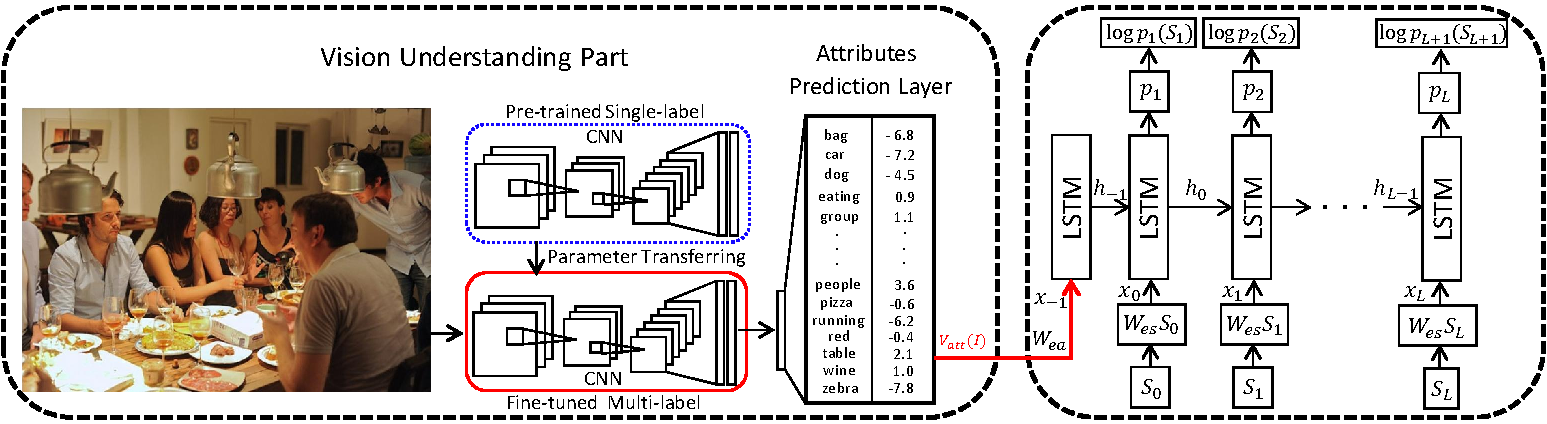
\includegraphics[width=0.85\textwidth]{./img/captioning_frame.pdf}\\
  \vspace{-5pt}
  \caption{Our attribute-based image captioning framework. The image analysis module learns a mapping between an image and the semantic attributes through a CNN. The language module learns a mapping from the attributes vector to a sequence of words using an LSTM. }
  \label{img:cap_frame}
  \vspace{-5pt}
\end{figure*}

\subsection{Visual Question Answering} Malinowski \etal \cite{malinowski2014multi}
may be the first to study the VQA problem. They proposed a method that combines semantic parsing and image segmentation with a Bayesian approach to sampling from nearest neighbors in the training set. %
Tu \etal~\cite{tu2014joint} built a query answering system based on a joint parse graph from text and videos. Geman \etal~\cite{geman2015visual} proposed an automatic `query generator' that is trained on annotated images and produces a sequence of binary questions from any given test image. Each of these approaches places significant limitations on the form of question that can be answered.

Most recently, inspired by the significant progress achieved using deep neural network models in both computer vision and natural language processing, an architecture which combines a CNN and RNN to learn the mapping from images to sentences has become the dominant trend. Both Gao \etal~\cite{gao2015you} and Malinowski \etal \cite{malinowski2015ask} used RNNs to encode the question and output the answer.  Whereas Gao \etal~\cite{gao2015you} used two networks, a separate encoder and decoder, Malinowski \etal \cite{malinowski2015ask} used a single network for both encoding and decoding. Ren \etal \cite{ren2015image} focused on questions with a single-word answer and formulated the task as a classification problem using an LSTM. %
Antol \etal \cite{antol2015vqa} proposed a large-scale open-ended VQA dataset based on COCO, which is called VQA. %
Inspired by Xu \etal \cite{xu2015show} who encode visual attention in the Image Captioning, \cite{zhu2015visual7w,xu2015ask,Chen2015ABC,Jiang2015compositional,andreas2015deep,yang2015stacked} propose to use the spatial attention to help answering visual questions. \cite{xu2015ask, yang2015stacked, Noh2015image}
formulate the VQA as a classification problem and restrict the answer only can be drawn from a fixed answer space. %

Our framework also exploits both CNN and RNNs, but in contrast to preceding approaches which use only image features extracted from a CNN in answering a question, we employ multiple sources, including image content, generated image captions and mined external knowledge, to feed to an RNN to answer questions. Large-scale Knowledge Bases (KBs), such as Freebase~\cite{bollacker2008freebase} and DBpedia~\cite{auer2007dbpedia}, have been used successfully in several natural language Question Answering (QA) systems~\cite{berant2013semantic,ferrucci2010building}. However, VQA systems exploiting KBs are still relatively rare.

%
Zhu \etal \cite{zhu2015building} used a hand-crafted KB primarily containing image-related information such as category labels, attribute labels and affordance labels, but also some quantities relating to their specific question format such as GPS coordinates and similar. %
Instead of building a problem-specific KB, we use a pre-built large-scale KB (DBpedia \cite{auer2007dbpedia}) from which we extract information using a standard RDF query language. DBpedia has been created by extracting structured information from Wikipedia, and is thus significantly larger and more general than a hand-crafted KB. Rather than having a user pose their question in a formal query language, our VQA system is able to encode questions written in natural language automatically.  This is achieved without manually specified formalization, but rather depends on processing a suitable training set. The result is a model which is very general in the forms of question that it will accept.
The quality of the information in the KB is one of the primary issues in this approach to VQA. The problem is that KBs constructed by analysing Wikipedia and similar are patchy and inconsistent at best, and hand-curated KBs are inevitably very topic specific. Using visually-sourced information is a promising approach to solve this problem~\cite{Lin_2015_CVPR, Sadeghi_2015_CVPR}, but has a way to go before it might be usefully applied within our approach. After inspecting the database shows that the ‘comment’ field is the most generally informative about an attribute, as it contains a general text description of it. We therefore find this is still a feasible solution. 
